\documentclass{article}

\usepackage[final]{neurips_2025}

% Replace NeurIPS conference footer with project info
\makeatletter
\renewcommand{\@noticestring}{Continuous Optimization Project, University of Basel, Spring Semester 2026.}
\makeatother

\usepackage[utf8]{inputenc}
\usepackage[T1]{fontenc}
\usepackage{hyperref}
\usepackage{url}
\usepackage{booktabs}
\usepackage{amsmath,amssymb,mathtools}
\usepackage{graphicx}
\usepackage{subcaption}
\usepackage{microtype}
\usepackage[section]{placeins}

\newcommand{\R}{\mathbb{R}}
\newcommand{\E}{\mathbb{E}}
\newcommand{\norm}[1]{\left\lVert #1 \right\rVert}

\title{Adaptive First-Order Methods for Logistic Objectives\\
and Non-Convex Reference Landscapes}

\author{
  Erion Krasniqi \quad Denis Mustafa Xhabrahimi \\
  University of Basel\\
  Continuous Optimization Project, Spring Semester 2026
}

\begin{document}
\maketitle

\begin{abstract}
Adaptive first-order methods modify the effective step size using the observed gradient history and are widely used in large-scale machine learning. This report compares stochastic gradient descent (SGD), Adagrad, AdaGrad-Norm, RMSprop, and Adam on two classification datasets, A9a and MNIST, using logistic and softmax cross-entropy objectives. We additionally evaluate logistic regression with the non-convex regularizer specified in the project description and include two controlled reference baselines: the Rosenbrock function, which exposes curved non-convex geometry, and full-batch L-BFGS as a quasi-Newton reference. Across the classification tasks, adaptive methods mainly improve the speed of optimization; final test accuracies are close across optimizers. The Rosenbrock benchmark makes Adam's advantage from momentum and adaptive coordinate scaling visible, while L-BFGS illustrates the behavior of a stronger deterministic full-batch method that is not directly comparable to mini-batch stochastic methods.
\end{abstract}

\section{Introduction}
Gradient-based optimization methods iterate
\begin{equation}
    w_{t+1}=w_t-\eta_t g_t,
\end{equation}
where $g_t$ is a gradient or stochastic gradient estimate. The practical difficulty is the choice of step size. A fixed learning rate can be too large in steep directions and too small in flat directions, especially in high-dimensional or sparse problems. Adaptive methods address this by scaling the update according to the trajectory of past gradients. This project studies the behavior of four adaptive methods, Adagrad, AdaGrad-Norm, RMSprop, and Adam, compared with SGD.

The project has two goals. First, we survey the mathematical update rules and qualitative differences between the methods. Second, we implement them in NumPy and compare their convergence on A9a and MNIST. Since the required logistic and softmax objectives are relatively well behaved, we also include a two-dimensional Rosenbrock benchmark to visualize a genuinely curved non-convex landscape. Finally, we add L-BFGS as a selected full-batch quasi-Newton reference, following the quasi-Newton framework surveyed by Xu and Zhang~\citep{xu2001survey}.

\section{Related Work and Methods}
\subsection{SGD}
Stochastic gradient descent uses a single global learning rate:
\begin{equation}
    w_{t+1}=w_t-\eta g_t.
\end{equation}
It is cheap per iteration and memory efficient, but sensitive to the learning rate and unable to adapt per coordinate.

\subsection{Adagrad}
Adagrad accumulates squared gradients coordinate-wise~\citep{duchi2011adaptive}:
\begin{equation}
    G_t=G_{t-1}+g_t\odot g_t,
\end{equation}
\begin{equation}
    w_{t+1}=w_t-\eta \frac{g_t}{\sqrt{G_t}+\epsilon}.
\end{equation}
Coordinates with large historical gradients receive smaller effective steps. This is useful for sparse features but the accumulated denominator can grow monotonically, causing steps to decay.

\subsection{AdaGrad-Norm}
AdaGrad-Norm replaces coordinate-wise accumulation by a single scalar accumulator~\citep{ward2020adagrad}:
\begin{equation}
    b_t^2=b_{t-1}^2+\norm{g_t}^2,
\end{equation}
\begin{equation}
    w_{t+1}=w_t-\frac{\eta}{b_t+\epsilon}g_t.
\end{equation}
It retains adaptive scaling and admits sharp convergence guarantees over non-convex landscapes, but lacks per-coordinate adaptation.

\subsection{RMSprop}
RMSprop uses an exponential moving average of squared gradients:
\begin{equation}
    v_t=\rho v_{t-1}+(1-\rho)g_t\odot g_t,
\end{equation}
\begin{equation}
    w_{t+1}=w_t-\eta\frac{g_t}{\sqrt{v_t}+\epsilon}.
\end{equation}
Unlike Adagrad, it forgets old gradients and can react faster when the local geometry changes. The method is widely used but is mostly heuristic from a convergence-theory perspective~\citep{ruder2016overview}.

\subsection{Adam}
Adam combines momentum with RMSprop-style scaling~\citep{kingma2014adam}:
\begin{align}
    m_t &= \beta_1 m_{t-1}+(1-\beta_1)g_t,\\
    v_t &= \beta_2 v_{t-1}+(1-\beta_2)g_t\odot g_t.
\end{align}
The bias-corrected moments are
\begin{equation}
    \hat m_t = \frac{m_t}{1-\beta_1^t},\qquad
    \hat v_t = \frac{v_t}{1-\beta_2^t},
\end{equation}
and the update is
\begin{equation}
    w_{t+1} = w_t-\eta \frac{\hat m_t}{\sqrt{\hat v_t}+\epsilon}.
\end{equation}
The first moment smooths the direction, while the second moment rescales coordinates. Reddi et al.~\citep{reddi2018convergence} showed that Adam can fail to converge in certain settings and proposed AMSGrad as a fix.

\subsection{L-BFGS Reference}
Quasi-Newton methods approximate curvature information using gradients and function values. In the classical BFGS form, the approximation $B_k$ to the Hessian is updated so that it satisfies the secant equation
\begin{equation}
    B_{k+1}s_k = y_k,\qquad
    s_k=x_{k+1}-x_k,\quad y_k=\nabla f(x_{k+1})-\nabla f(x_k).
\end{equation}
This condition incorporates local curvature without explicitly forming the true Hessian. Limited-memory BFGS stores only a small number of recent $(s_k,y_k)$ pairs, which makes it practical for larger models while preserving the main quasi-Newton idea. We use L-BFGS-B from SciPy as a full-batch reference method for selected objectives. Because each L-BFGS iteration uses full objective and gradient evaluations, it is not treated as a mini-batch competitor; instead it contextualizes the stochastic first-order results.

\section{Experimental Setup}
\subsection{Datasets}
We use two LIBSVM datasets. A9a is a binary classification problem with 32,561 training samples and 123 sparse features; labels are represented as $y_i\in\{-1,+1\}$. MNIST is a ten-class classification problem with 60,000 training samples and 780 features in the LIBSVM version used here.

\subsection{Objectives}
For A9a, the convex logistic objective is
\begin{equation}
    L(w)=\frac{1}{n}\sum_{i=1}^n \log(1+\exp(-y_i x_i^\top w)).
\end{equation}
We also evaluate the non-convex regularized objective from Reddi et al.~\citep{reddi2016fast}:
\begin{equation}
    L_{\mathrm{nc}}(w)=L(w)+\lambda\sum_j\frac{\alpha w_j^2}{1+\alpha w_j^2},
    \qquad \lambda=10^{-2},\quad \alpha=1.
\end{equation}
For MNIST, we use linear softmax regression with cross-entropy loss.

\subsection{Gradients}
For binary logistic regression, with $z_i=y_i x_i^\top w$, the gradient of the average loss is
\begin{equation}
    \nabla L(w)= -\frac{1}{n}\sum_{i=1}^n y_i x_i \,\sigma(-z_i),
    \qquad \sigma(t)=\frac{1}{1+\exp(-t)}.
\end{equation}
The non-convex regularizer is separable across coordinates. For
\begin{equation}
    r_j(w_j)=\frac{\alpha w_j^2}{1+\alpha w_j^2},
\end{equation}
the derivative is
\begin{equation}
    r_j'(w_j)=\frac{2\alpha w_j}{(1+\alpha w_j^2)^2}.
\end{equation}
This derivative is linear near zero but decays for large $|w_j|$, which makes the regularization term non-convex and qualitatively different from standard $\ell_2$ regularization. For MNIST, if $P=\mathrm{softmax}(XW)$ and $Y$ is the one-hot label matrix, then the full gradient is $X^\top(P-Y)/n$.

\subsection{Reference Objective}
To isolate non-convex geometry, we use the Rosenbrock function~\citep{rosenbrock1960automatic}
\begin{equation}
    f(x,y)=(1-x)^2+100(y-x^2)^2,
\end{equation}
which has a narrow curved valley and global minimum at $(1,1)$. This benchmark is not an additional dataset experiment; it is a controlled reference for optimizer trajectories.

\subsection{Protocol}
All stochastic optimizers are implemented from scratch in NumPy. We use mini-batches, report training loss and test accuracy, and average stochastic runs over three seeds. A9a is trained with batch size $128$ for 10 epochs, while MNIST is trained with batch size $256$ for 15 epochs. Hyperparameters are fixed after preliminary tuning: on A9a, SGD and Adagrad use $\eta=10^{-1}$, AdaGrad-Norm uses $\eta=1$, RMSprop uses $\eta=10^{-2}$, and Adam uses $\eta=5\cdot 10^{-3}$. On MNIST, the corresponding values are $5\cdot10^{-2}$, $10^{-1}$, $5\cdot10^{-1}$, $10^{-3}$, and $10^{-3}$.

For the Rosenbrock reference, all methods start from the same initial point and are run for a fixed iteration budget so that trajectory differences are visible. For L-BFGS, we use deterministic full-batch objective and gradient evaluations. This distinction matters: one L-BFGS iteration can be substantially more expensive than one mini-batch first-order update, so the comparison should be read as a reference comparison rather than as a direct per-iteration race.

\section{Results}
\subsection{Classification Objectives}
\begin{figure}[t]
    \centering
    \begin{subfigure}{0.49\linewidth}
        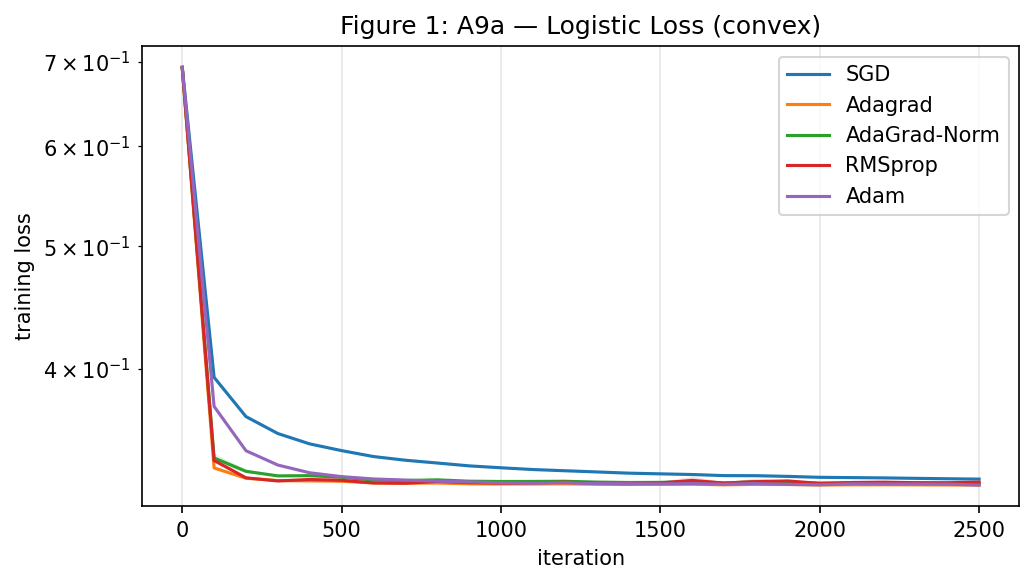
\includegraphics[width=\linewidth]{figures/a9a_logistic_loss.png}
        \caption{A9a logistic loss}
    \end{subfigure}
    \hfill
    \begin{subfigure}{0.49\linewidth}
        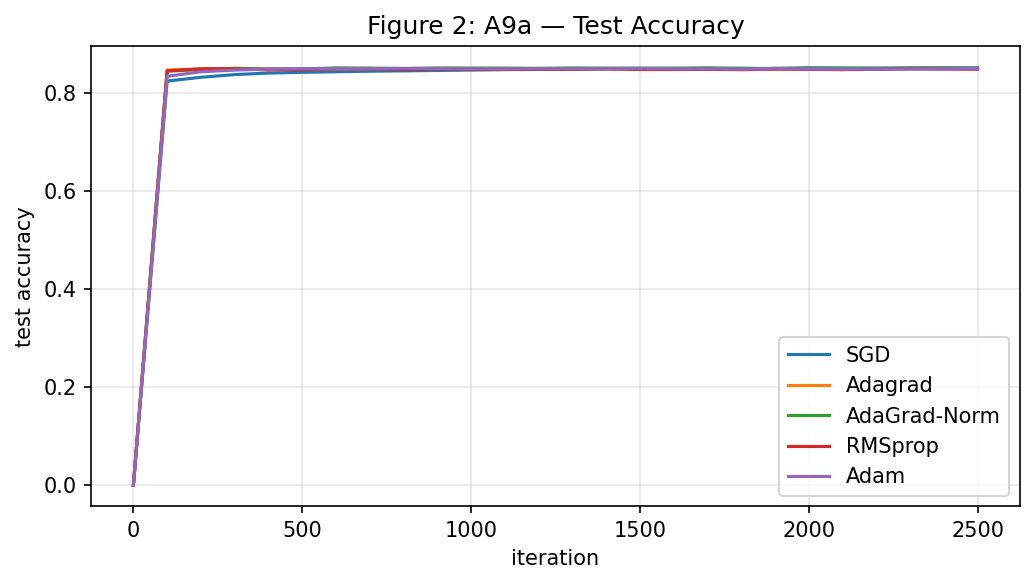
\includegraphics[width=\linewidth]{figures/a9a_logistic_acc.png}
        \caption{A9a test accuracy}
    \end{subfigure}
    \vspace{0.35em}
    \begin{subfigure}{0.49\linewidth}
        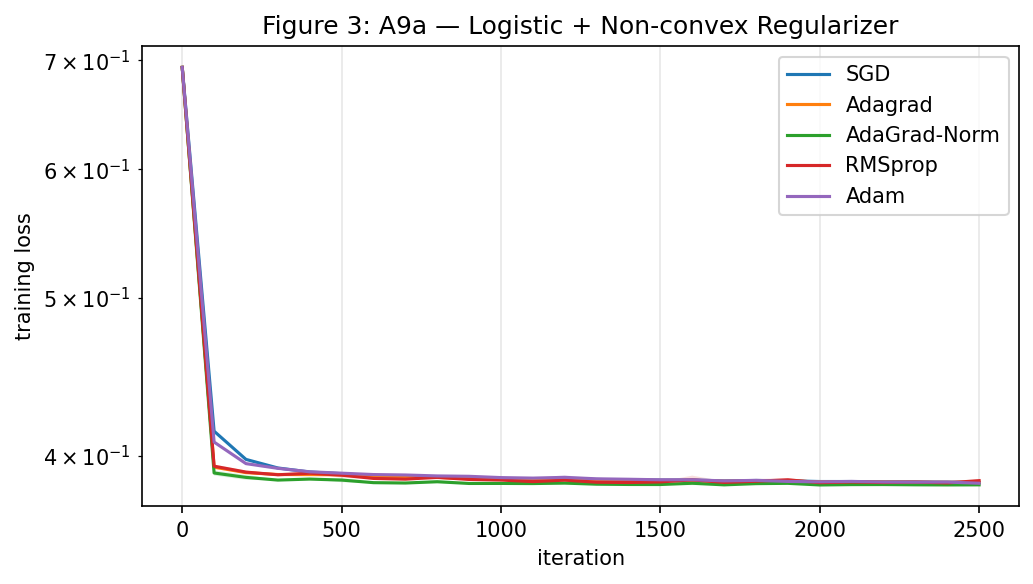
\includegraphics[width=\linewidth]{figures/a9a_nonconvex_loss.png}
        \caption{A9a non-convex loss}
    \end{subfigure}
    \hfill
    \begin{subfigure}{0.49\linewidth}
        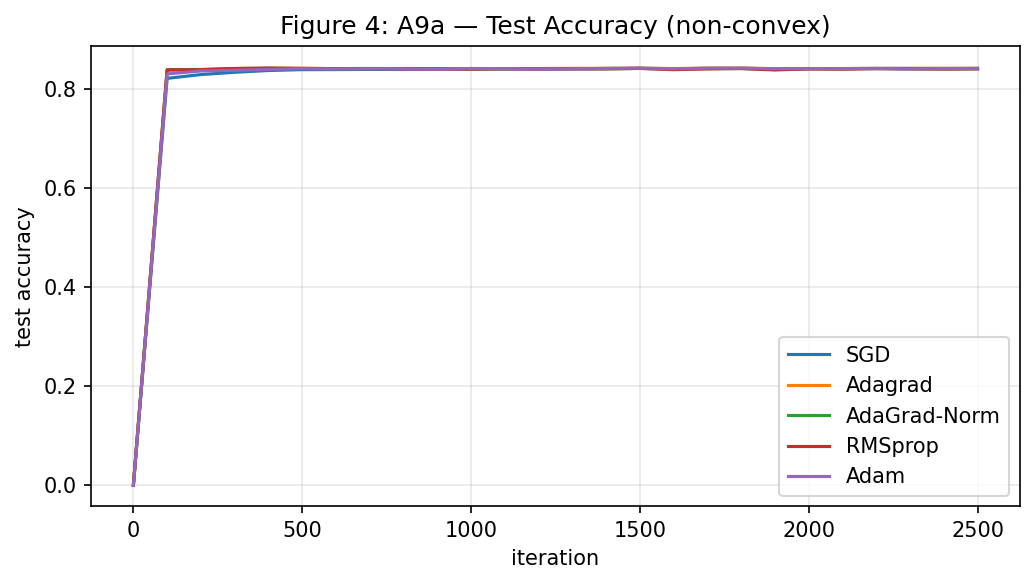
\includegraphics[width=\linewidth]{figures/a9a_nonconvex_acc.png}
        \caption{A9a non-convex accuracy}
    \end{subfigure}
    \caption{A9a results. Adaptive methods reduce loss faster on convex logistic regression, while final test accuracy remains similar. The non-convex regularizer raises the objective value but does not substantially change the optimizer ranking at $\lambda=10^{-2}$.}
    \label{fig:a9a}
\end{figure}

Figure~\ref{fig:a9a} shows that adaptive methods decrease the loss faster in early iterations, while final accuracies are nearly identical ($84$--$85\%$). Adding the non-convex regularizer raises the objective but does not substantially change the optimizer ranking at $\lambda=10^{-2}$.

\begin{figure}[t]
    \centering
    \begin{subfigure}{0.49\linewidth}
        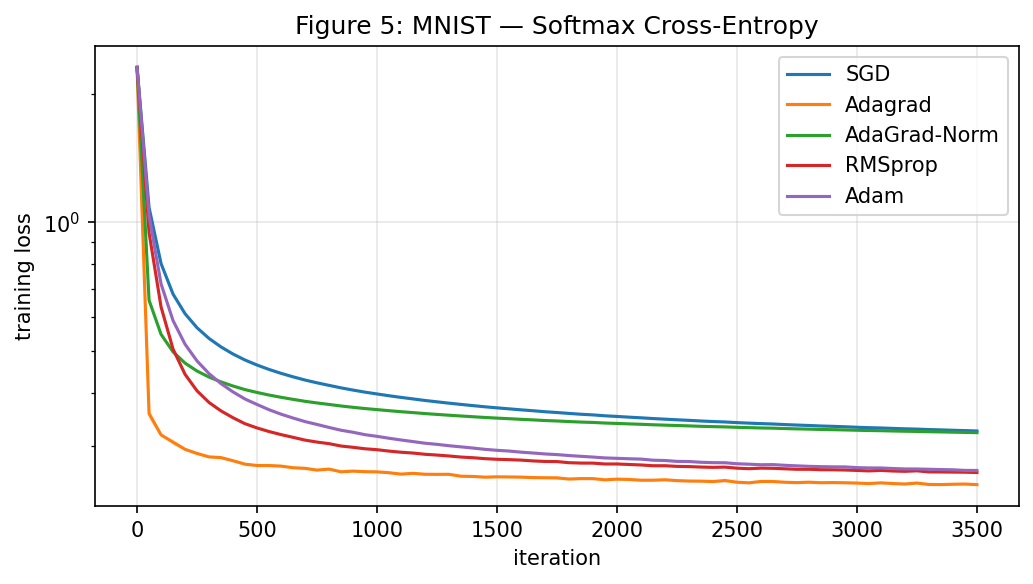
\includegraphics[width=\linewidth]{figures/mnist_loss.png}
        \caption{MNIST softmax loss}
    \end{subfigure}
    \hfill
    \begin{subfigure}{0.49\linewidth}
        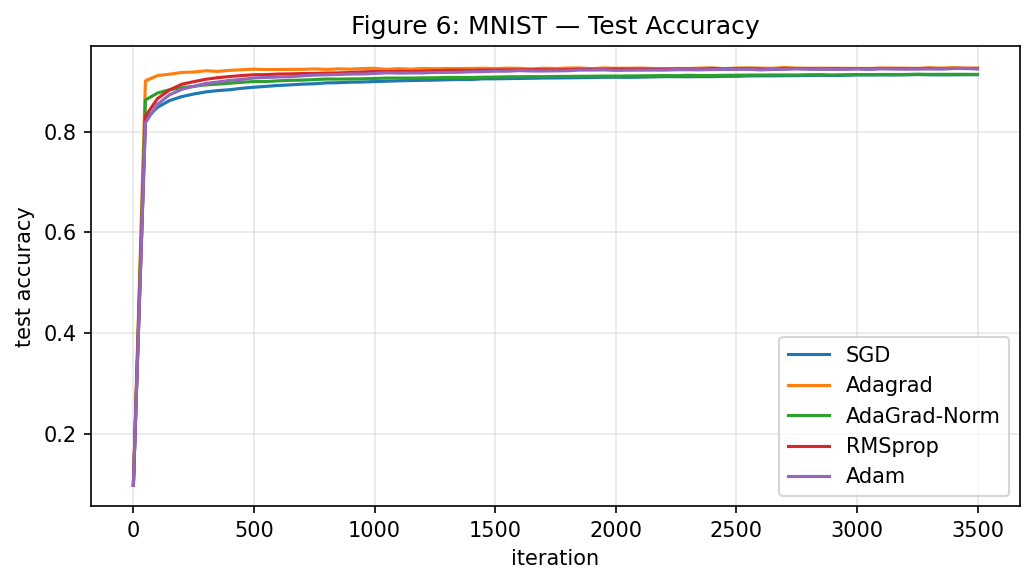
\includegraphics[width=\linewidth]{figures/mnist_acc.png}
        \caption{MNIST test accuracy}
    \end{subfigure}
    \caption{MNIST is higher-dimensional. Per-coordinate adaptation is more useful here: Adagrad reaches the lowest final loss, while RMSprop and Adam are close behind.}
    \label{fig:mnist}
\end{figure}

On MNIST (Figure~\ref{fig:mnist}), Adagrad achieves the best final loss, with RMSprop and Adam close behind. Final accuracies differ only modestly, but adaptive methods reach good performance earlier.

\begin{table}[t]
    \centering
    \caption{Final training loss and test accuracy. Values for stochastic methods are means over three seeds. L-BFGS is a full-batch quasi-Newton reference and was only run on selected objectives.}
    \label{tab:summary}
    \small
    \begin{tabular}{lrrrrrr}
        \toprule
        Optimizer & A9a loss & A9a acc & NC loss & NC acc & MNIST loss & MNIST acc\\
        \midrule
        SGD          & 0.3270 & 0.8516 & 0.3851 & 0.8425 & 0.3254 & 0.9134\\
        Adagrad      & 0.3234 & 0.8495 & 0.3850 & 0.8425 & \textbf{0.2438} & \textbf{0.9266}\\
        AdaGrad-Norm & 0.3244 & 0.8506 & \textbf{0.3838} & 0.8416 & 0.3225 & 0.9140\\
        RMSprop      & 0.3252 & 0.8488 & 0.3861 & 0.8416 & 0.2603 & 0.9257\\
        Adam         & 0.3234 & 0.8500 & 0.3847 & 0.8423 & 0.2631 & 0.9247\\
        L-BFGS$^\ast$ & \textbf{0.3226} & 0.8499 & 0.3835 & 0.8420 & -- & --\\
        \bottomrule
    \end{tabular}
    \vspace{0.25em}

    \footnotesize{$^\ast$Full-batch quasi-Newton reference; not directly comparable to mini-batch stochastic methods.}
\end{table}

\subsection{Robustness and Wall-Clock Time}
\begin{figure}[t]
    \centering
    \begin{subfigure}{0.49\linewidth}
        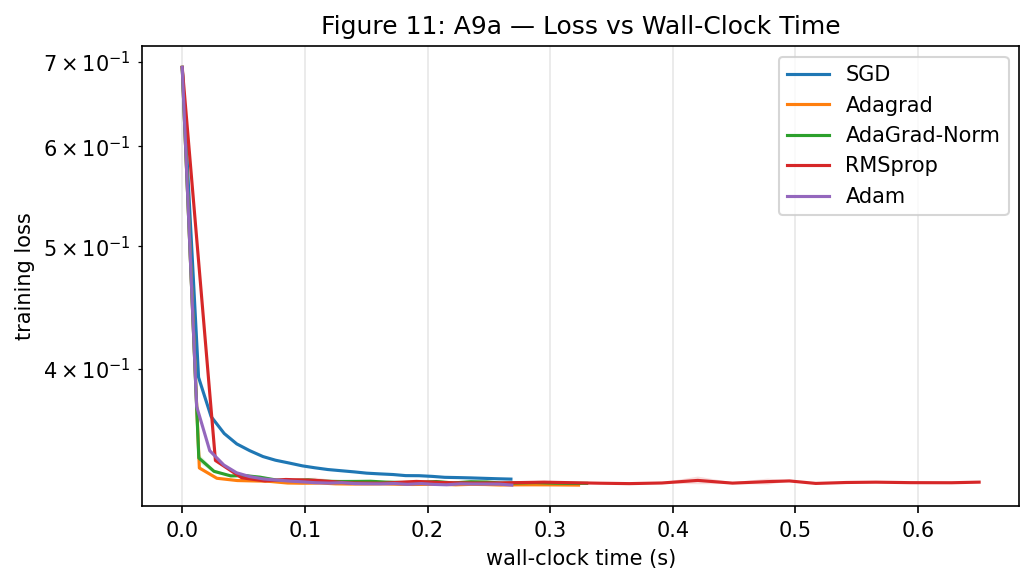
\includegraphics[width=\linewidth]{figures/wallclock_a9a.png}
        \caption{A9a wall-clock}
    \end{subfigure}
    \hfill
    \begin{subfigure}{0.49\linewidth}
        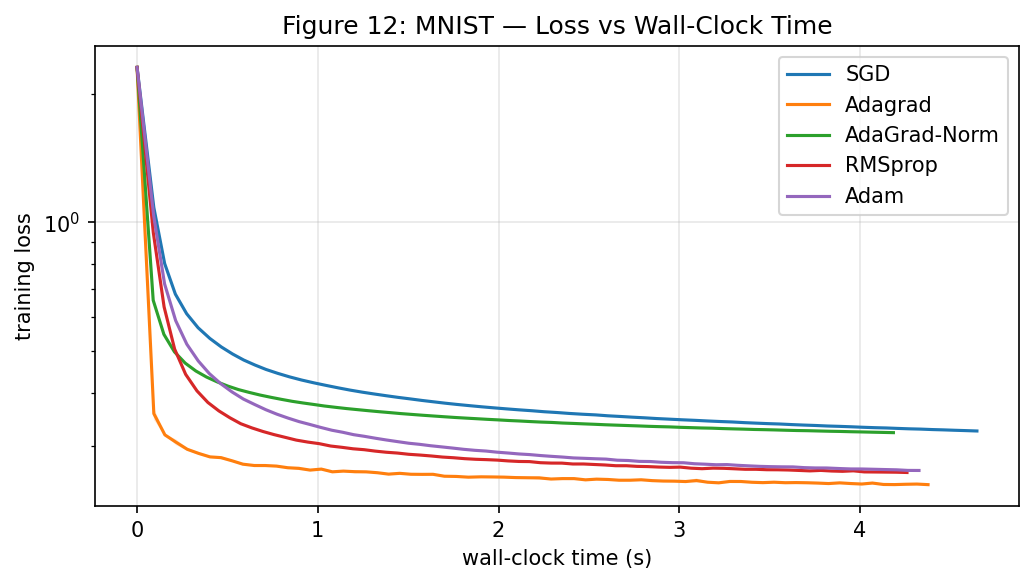
\includegraphics[width=\linewidth]{figures/wallclock_mnist.png}
        \caption{MNIST wall-clock}
    \end{subfigure}
    \caption{Adaptive methods have slightly more per-step overhead, but they often reach low loss earlier in actual runtime because they need fewer effective optimization steps.}
    \label{fig:wallclock}
\end{figure}

Figure~\ref{fig:wallclock} shows that the per-step overhead of adaptive methods is small relative to their benefit from faster loss reduction. On both datasets, adaptive methods reach their final loss faster in wall-clock time.

\begin{figure}[t]
    \centering
    \begin{subfigure}{0.70\linewidth}
        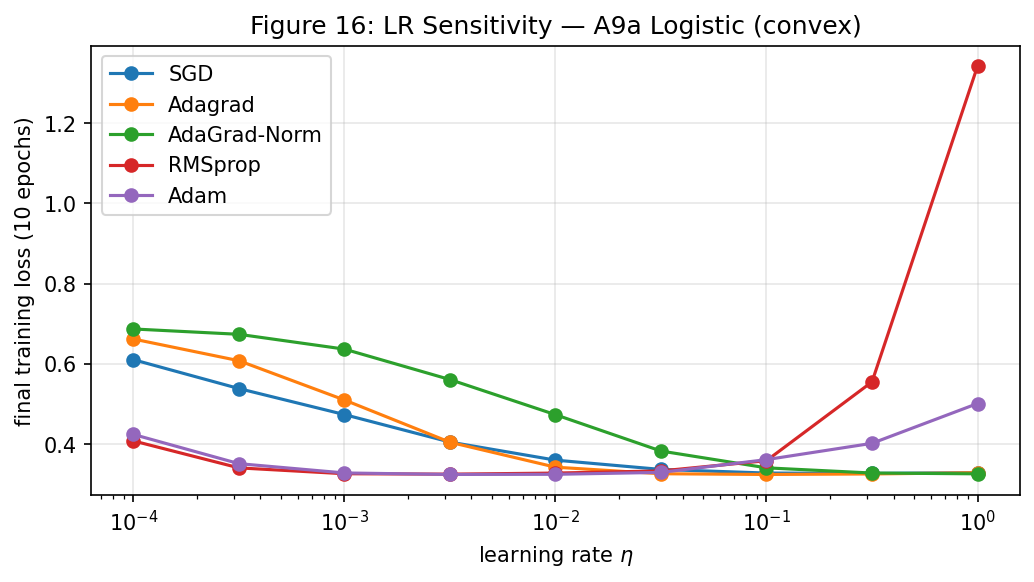
\includegraphics[width=\linewidth]{figures/lr_sweep_a9a.png}
        \caption{Learning-rate sensitivity}
    \end{subfigure}
    \vspace{0.4em}
    \begin{subfigure}{0.70\linewidth}
        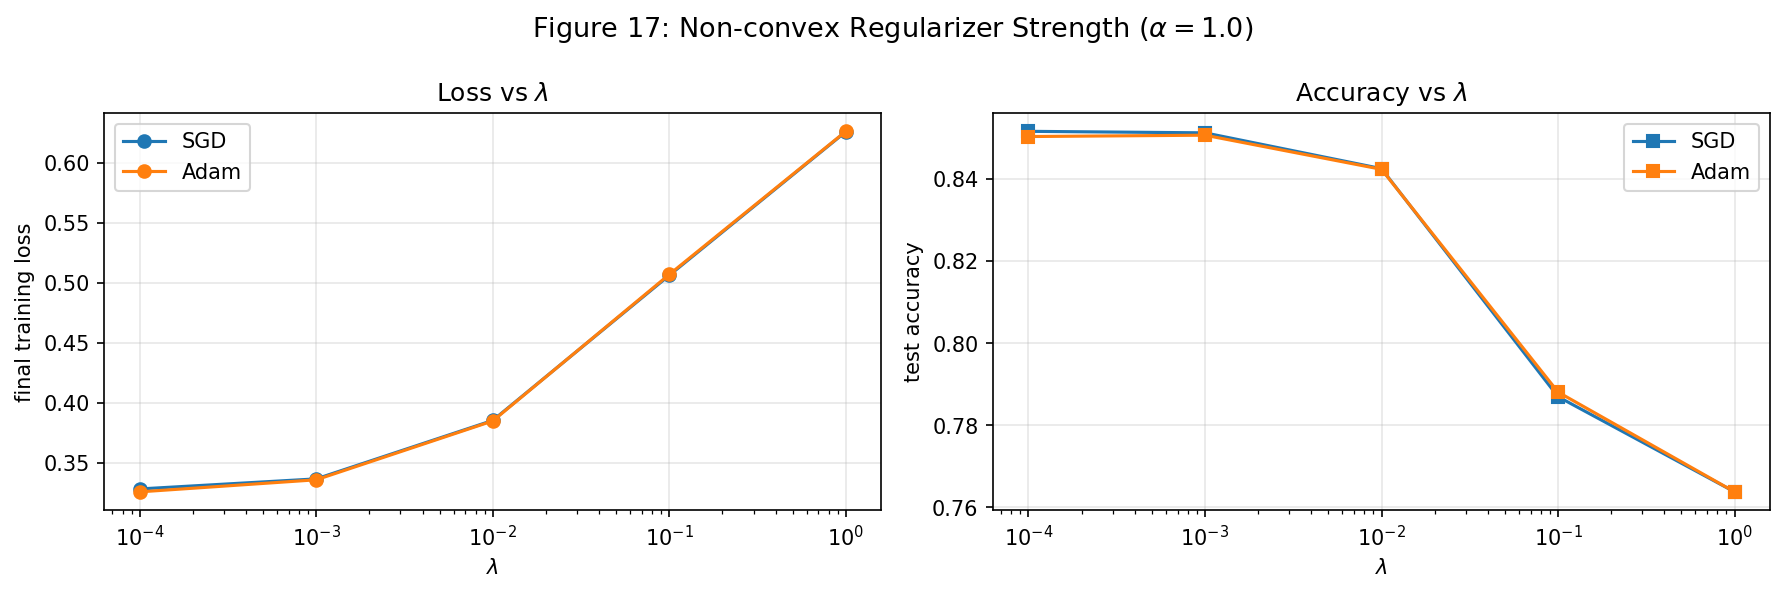
\includegraphics[width=\linewidth]{figures/lambda_sweep.png}
        \caption{Regularization strength}
    \end{subfigure}
    \caption{Sensitivity experiments. The learning-rate sweep illustrates optimizer robustness, while the $\lambda$ sweep shows when the non-convex regularizer starts to dominate.}
    \label{fig:sensitivity}
\end{figure}

The learning-rate sweep in Figure~\ref{fig:sensitivity} shows that SGD and AdaGrad-Norm are predictable over a broad range, while RMSprop becomes unstable for large rates. Adaptivity reduces, but does not remove, the need for tuning. The $\lambda$ sweep confirms that for small $\lambda$ the regularizer changes the objective only mildly; for larger $\lambda$ it dominates and accuracy drops, motivating our use of Rosenbrock as the clearer non-convex reference.

\subsection{Gradient Norms and Reference Benchmarks}
\begin{figure}[t]
    \centering
    \begin{subfigure}{0.49\linewidth}
        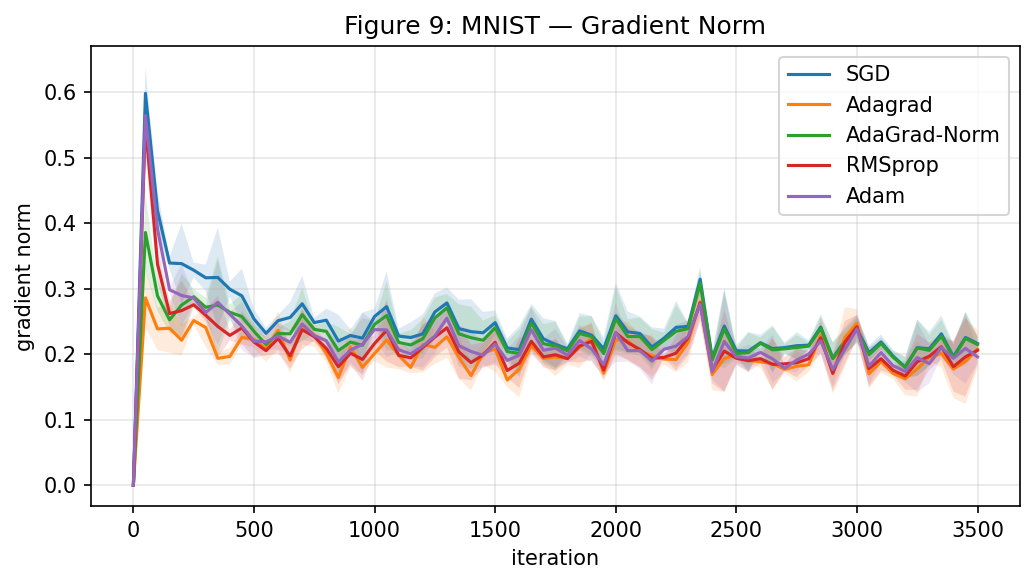
\includegraphics[width=\linewidth]{figures/mnist_gradnorm.png}
        \caption{MNIST gradient norms}
    \end{subfigure}
    \hfill
    \begin{subfigure}{0.49\linewidth}
        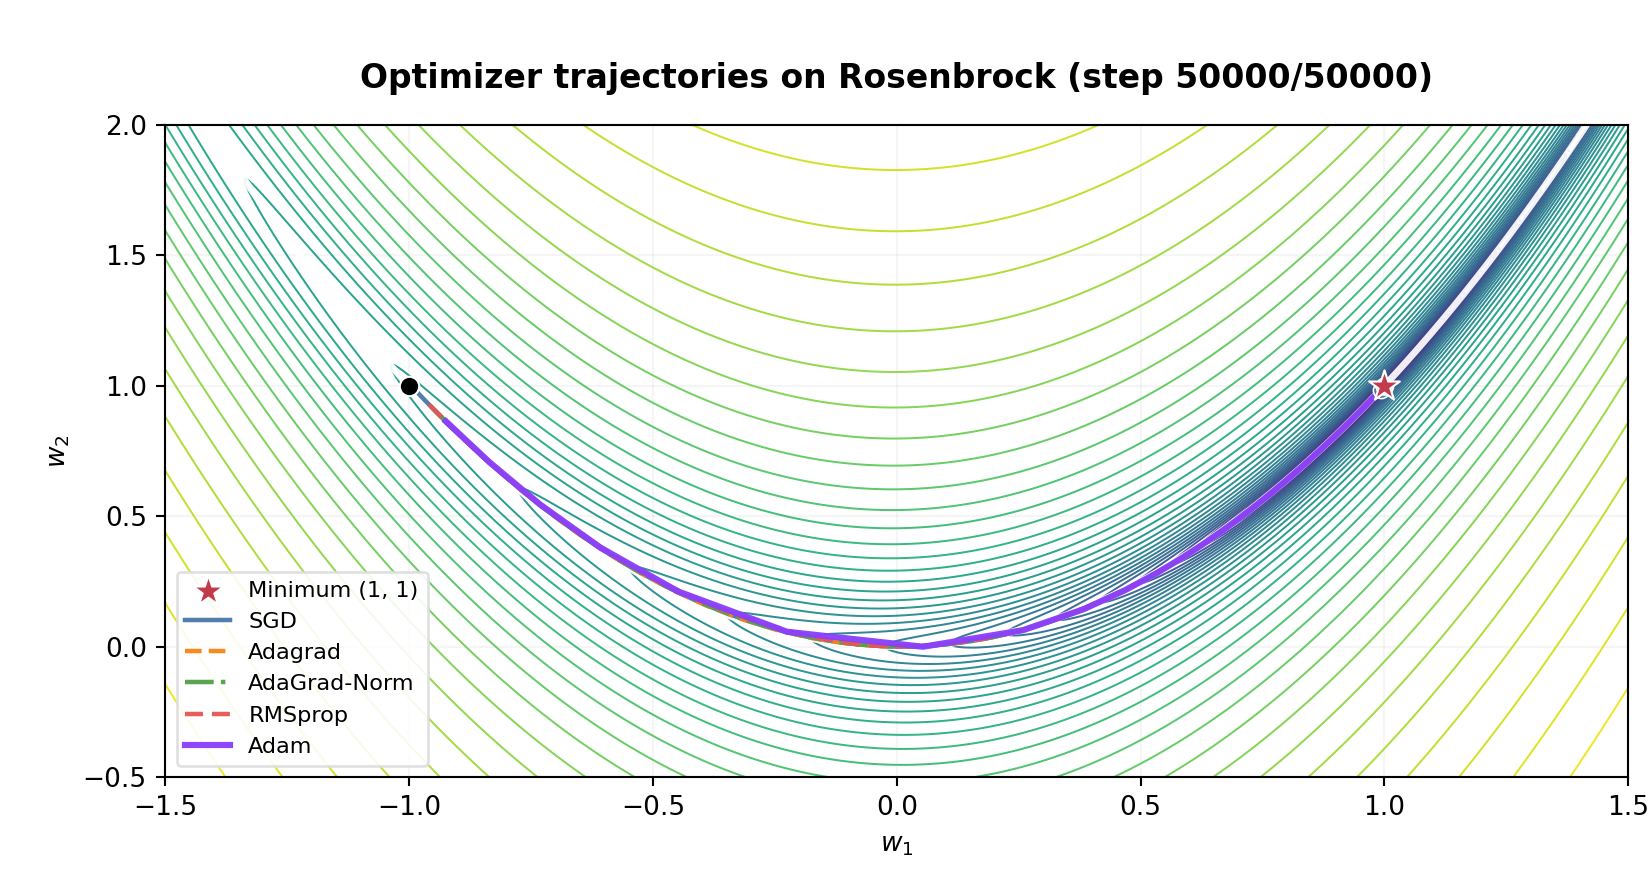
\includegraphics[width=\linewidth]{figures/rosenbrock_final.png}
        \caption{Rosenbrock trajectories}
    \end{subfigure}
    \caption{Gradient norms explain the faster early progress of adaptive methods. Rosenbrock highlights Adam's advantage on a curved non-convex valley.}
    \label{fig:diagnostics}
\end{figure}

Gradient norms (Figure~\ref{fig:diagnostics}) show that adaptive methods normalize large early gradients and maintain progress as gradients shrink. On Rosenbrock, Adam's combination of momentum and coordinate-wise scaling is clearly visible: SGD requires many more iterations to follow the curved valley.

\begin{figure}[t]
    \centering
    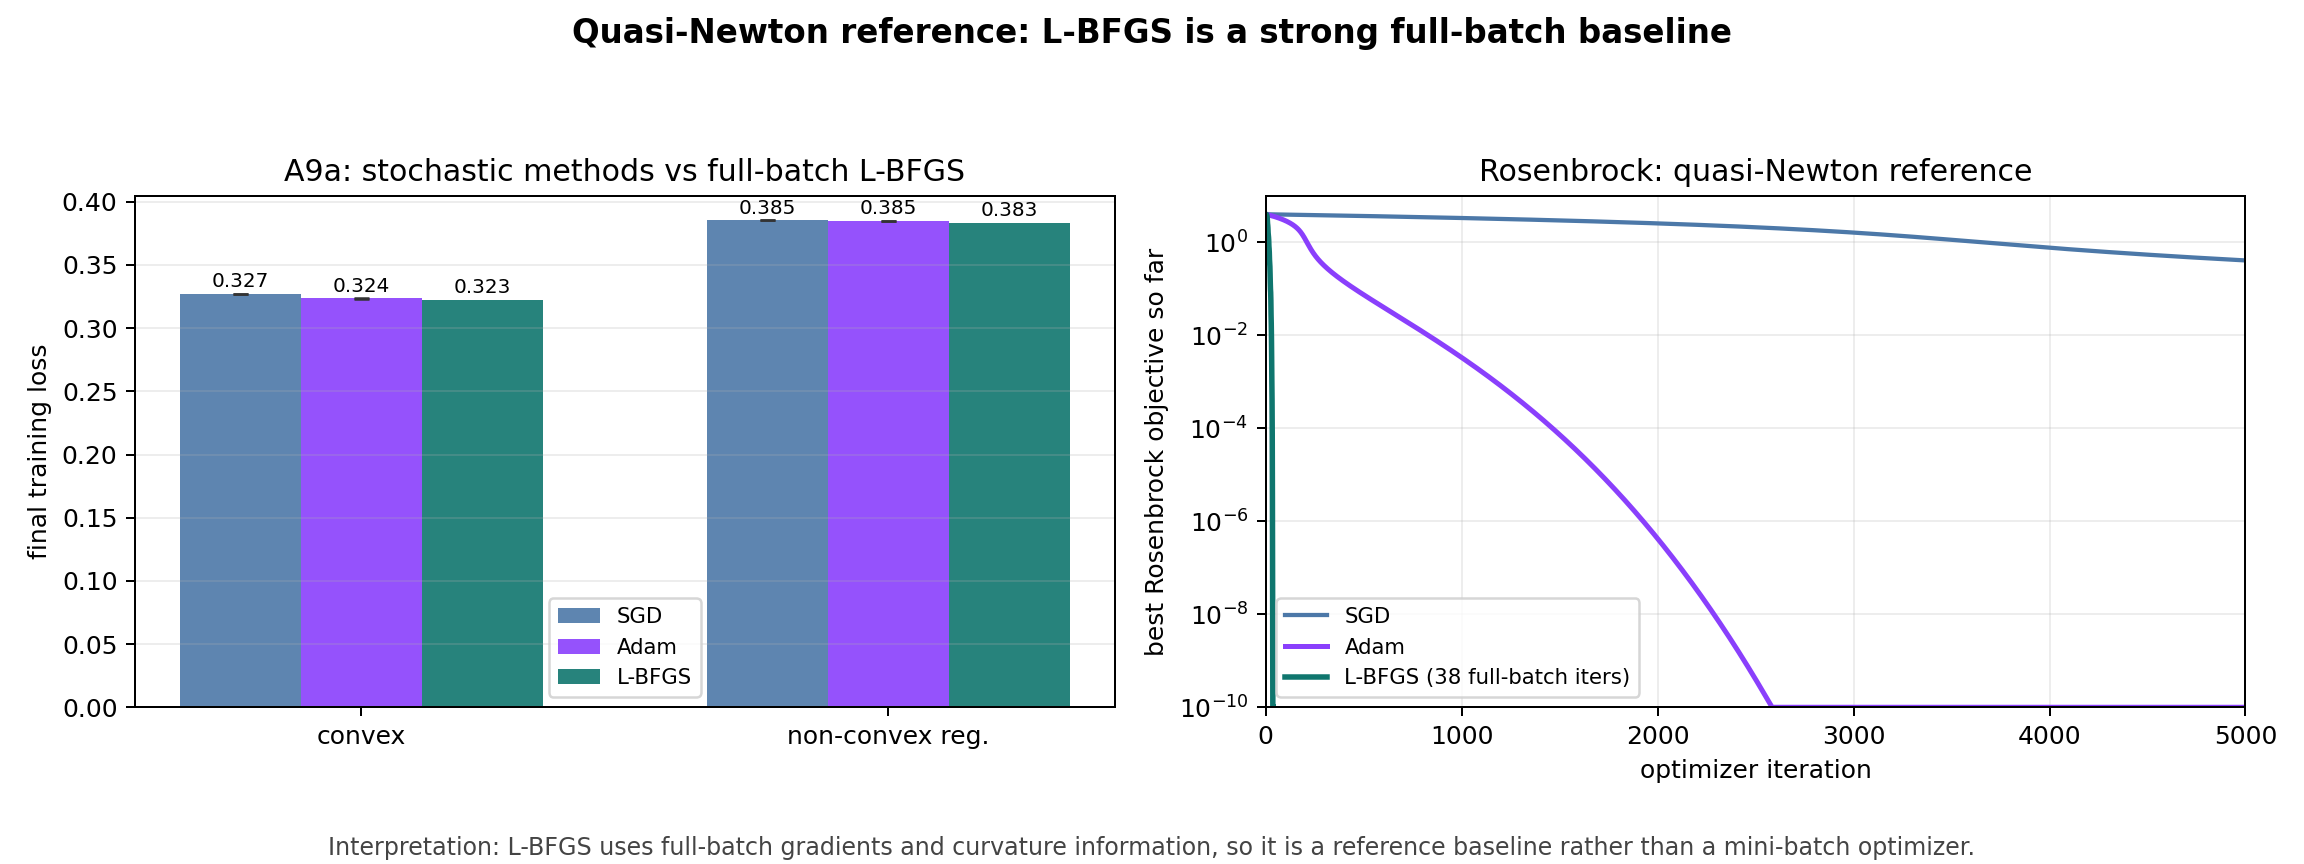
\includegraphics[width=0.85\linewidth]{figures/lbfgs_reference.png}
    \caption{L-BFGS reference. On A9a, L-BFGS reaches comparable final losses. On Rosenbrock, it solves the benchmark in 38 full-batch iterations, illustrating why it should be interpreted as a separate deterministic reference rather than as a mini-batch competitor.}
    \label{fig:lbfgs}
\end{figure}

Figure~\ref{fig:lbfgs} shows that L-BFGS obtains the best final loss on convex A9a and solves Rosenbrock in very few iterations, highlighting the difference between curvature-based deterministic methods and stochastic adaptive methods.

\section{Discussion and Limitations}
The main empirical result is consistent across datasets: adaptive methods improve convergence speed more than final classification accuracy. The strongest benefit appears in early loss reduction and in the ability to handle coordinate-wise gradient heterogeneity.

The comparison separates three notions that are often conflated: iteration efficiency, runtime efficiency, and final generalization. Adagrad and Adam can look strong per iteration because they rescale coordinates; in wall-clock time, this advantage remains only if the extra arithmetic is cheaper than the saved iterations. Final test accuracy is a different question: once the linear models are sufficiently optimized, all methods reach similar decision boundaries.

The non-convex regularizer from the project description has limited practical effect at $\lambda=10^{-2}$. For this dataset and regularization strength, the landscape remains too well behaved to show a dramatic Adam advantage. Rosenbrock complements the dataset experiments by isolating the relevant geometry.

The quasi-Newton reference should be interpreted carefully. L-BFGS uses curvature information and full-batch gradients, so it is expected to perform very well on smooth objectives. Its role is not to replace adaptive first-order methods, but to contextualize stochastic results with a deterministic baseline.

Limitations include: manually tuned hyperparameters, L-BFGS evaluated only on selected objectives, and the use of linear models that do not fully capture deep non-convex loss surfaces.

\section{Conclusion}
We implemented and compared SGD, Adagrad, AdaGrad-Norm, RMSprop, and Adam on A9a and MNIST. Adaptive methods consistently accelerated early optimization, while final test accuracies remained similar. Adagrad performed especially well on MNIST, indicating that per-coordinate scaling is useful in higher-dimensional classification. The required non-convex regularized logistic objective did not strongly separate the optimizers at moderate regularization strength. A controlled Rosenbrock benchmark made Adam's advantage on curved non-convex geometry clearer, and L-BFGS provided a useful but separate quasi-Newton reference. Overall, the practical benefit of adaptive methods in our experiments is speed and robustness of optimization rather than substantially better final generalization.

\bibliographystyle{plainnat}
\bibliography{references}

\end{document}
